\chapter{Implementatie}

\label{Chapter6}

Dit hoofdstuk gaat over de deelvraag \enquote{\deelimplementatie}. In dit hoofdstuk staat de bijbehorende gedachtegang met referenties naar de code en ontwerpen in bijlage \ref{BijlageCode}.

\section{Feature-environments} \label{implementatieFeatureEnvs}

Alle code en ontwerpen voor feature-environments zijn te vinden in bijlage \ref{CodeFeatureEnvironments}. Om te helpen met de ontwikkelfase en documentatie zijn allereerst twee diagrammen ontworpen. Een component diagram voor de Docker containers samen met de reverse proxy (figuur \ref{traefikinfrastructure}), dit is een bijgewerkte versie van figuur \ref{fig:infra}, en daarnaast is een activity diagram ontworpen om de deployment workflow te visualiseren (figuur \ref{activitydiagram}).

\begin{figure}[H]
	\centering
	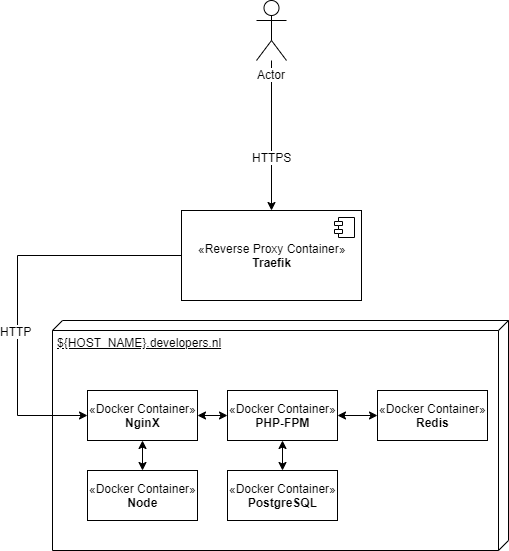
\includegraphics[width=9cm]{Figures/Traefik}
	\decoRule
	\caption[Traefik Infrastructure]{Nieuwe infrastructuur met Traefik reverse proxy}
	\label{traefikinfrastructure}
\end{figure}

\begin{figure}[H]
	\centering
	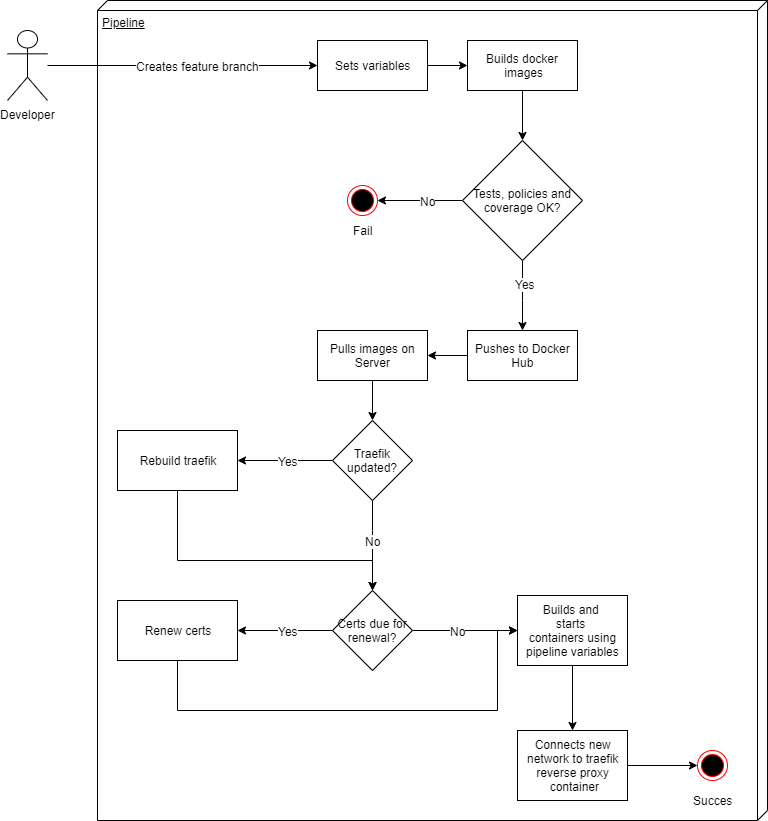
\includegraphics[width=13cm]{Figures/Activitydiagram}
	\decoRule
	\caption[Pipeline Activity Diagram]{Activity Diagram voor de pipeline}
	\label{activitydiagram}
\end{figure}

Hierna is de Docker opstelling gemaakt voor Traefik. De bestaande drie Docker-compose bestanden zijn aangepast door de Nginx service labels te geven die zorgen voor de service-discovery van Traefik. Vervolgens zijn basis, productie, en development docker-compose bestanden aangemaakt voor Traefik. Het afhandelen van SSL in development gebeurt niet meer via Nginx maar via Traefik, daarom is de development\_ssl service hier naar verplaatst. Deze service is tevens ook aangepast om wildcard certificaten te genereren, en om niet meer afhankelijk te zijn van een image uit een derde partij. Hierdoor is ook de Nginx configuratie aangepast om de afhandeling van SSL niet meer te ondersteunen. Ook is een configuratiebestand voor traefik toegevoegd voor de TLS instellingen. Om de development omgeving te ondersteunen is de Makefile bijgewerkt en een script gemaakt om de omgeving op te zetten. Dit script gebruikt de development Docker-compose bestanden om de containers te draaien en verbind vervolgens Nginx met Traefik.

Traefik runt standaard als root, dit is geen best-practice voor het gebruiken van Docker Containers \parencite{DockerBestPractices}. Daarom is een Dockerfile toegevoegd die verder bouwt op de Traefik image. Deze dockerfile maakt een user en group aan om deze vervolgens te gebruiken om het proces mee te runnen. Deze user en group komen overeen met users op de host machine, waardoor deze rechten heeft tot de Docker client certificaten.

Vervolgens is er een Ansible role ontwikkeld om de Docker Daemon te beveiligen via TLS\footnote{https://github.com/ansible/role-secure-docker-daemon is gebruikt voor inspiratie, maar omdat dit project erg verouderd is, is besloten om een verbeterde versie te ontwikkelen.}. Om te helpen bij de ontwikkeling is eerst een Vagrantfile toegevoegd om met Virtualbox lokaal de Ansible role te kunnen testen. Deze role genereert een Certificate Authority (CA), server, en client keys door middel van OpenSSL. Ook zorgt deze role er voor dat de Docker Daemon correct is ingesteld om deze certificaten te kunnen gebruiken, en dat de permissions van alle bestanden juist zijn ingesteld. De \texttt{daemon.json} wordt gevuld met variabelen uit Ansible door middel van een Jinja2 template. Er wordt gebruik gemaakt van Ansible-Vault om de passphrase van de certificaten veilig op te slaan.

Om de implementatie te deployen naar productie zijn de bestaande Ansible roles aangepast om gebruik te maken van de Traefik proxy en beveiligde Docker Daemon. In de \texttt{frontend-images} role is de Dockerfile toegevoegd met de relevante build arguments. De frontend role haalt de environment variabelen uit de Bitbucket Pipeline en parsed deze om zo de correcte subdomein, Fully Qualified Domain Name (FQDN), en network name te registreren. Deze worden gebruikt als variabelen in de docker-compose bestanden om zo de correcte subdomeinen aan te maken. Vervolgens worden de containers gebuild en Nginx aan de Traefik en PHP-FPM containers verbonden. Zodra de naam van de git branch geen \enquote{Feature/WEB-} bevat wordt er geen aparte feature-environment gebruikt voor de deployment.

De Bitbucket Pipeline is aangepast om Traefik te updaten bij een deployment of bootstrap.

\section{Codecov}
Code voor het implementeren is te zien in bijlage \ref{codecov}. Bitbucket en codecoverage environment variabelen moesten worden doorgegeven aan de Dockerfile van PHP-FPM door middel build arguments. Het builden van de Docker images gebeurt met Ansible. In de php7-fpm Dockerfile zijn de build arguments omgezet naar environment variablen, een aantal apk packages toegevoegd, en is het Codecov script toegevoegd. Er is een script geschreven om pcov te installeren zodat dit kan hergebruikt worden zowel in de \texttt{develop.sh} entrypoint als in de test-stage van de Dockerfile.

Om BitBucket een betere ondersteuning te geven met Codecov is een Pull-Request naar de Codecov-bash repository gemaakt. Deze is te zien op:\\ \texttt{https://github.com/codecov/codecov-bash/pull/225}. De maintainers van Codecov waren tevreden met deze verbeteringen en hebben de Pull-Request geaccepteerd en gemerged.

\section{Opschonen Docker images}
In het bestand \texttt{developers.nl/ansible/group\_vars/all.yml} is een variabele geplaatst om de images te filteren, images die ouder zijn dan 4 uur worden verwijderd.
\begin{minted}[linenos=true, bgcolor=codebg]{yaml}
image_delete_until_time: 4h
\end{minted}
\\In \texttt{developers.nl/ansible/deploy.yml} is een ansible taak geplaatst die gebruik maakt van de \texttt{docker\_prune} module, om zo alle dangling images te verwijderen.
\begin{minted}[linenos=true, bgcolor=codebg]{yaml}
- name: "Clean up images older than {{ image_delete_until_time }}"
  docker_prune:
    images: yes
    images_filters:
      dangling: false
      until: "{{ image_delete_until_time }}"
  register: prune_result
\end{minted}

\section{Policy as Code}

Implementatie van Open Policy Agent staat in Bijlage \ref{OPAImplementatie}. Er zijn verschillende locaties waar policies afgedwongen kunnen worden; build-time en run-time. Build-time policies kunnen bijvoorbeeld pipelines laten failen zodra er Docker images gebouwd worden met incorrecte poorten of met niet-toegestane users. Run-time policies kunnen draaiende containers evalueren of users managen. Voor deze eerste opzet wordt gekeken naar de user die een Docker commando uitvoert. Dit mogen alleen \texttt{runuser}, \texttt{developer} of \texttt{root} zijn. 

Voor het evalueren van build-time policies wordt gebuik gemaakt van de \texttt{openpolicyagent/opa} Docker image die het \texttt{eval} commando gebruikt. Deze container wordt gebuild in de Ansible role die alle Docker images voor de website build. Dit gebeurt door middel van de Ansible \texttt{docker\_container} module. Deze task faalt zodra de text \texttt{"allow": true} niet in de container stdout voorkomt. Voor deze eerste opzet is een policy aangemaakt die evalueert of 1 gelijk is aan 2. Als dat zo is, faalt de pipeline.

De run-time policy is geplaatst in de Ansible \texttt{secure-daemon} role. Meer informatie over deze role is te vinden in paragraaf \ref{implementatieFeatureEnvs}. Deze role configureert de Docker Daemon van verschillende users door een \texttt{config.json} te plaatsen in de home directory van de toegestane users. De JSON wordt gevuld met variabelen uit Ansible, door middel van een Jinja2 template. Deze configuratie stuurt een HttpHeader mee met uitgevoerde Docker commando's die OPA vertelt wie de uitvoerende user is. OPA evalueert hierna of deze user rechten heeft om dit commando uit te voeren door middel van de \texttt{openpolicyagent/opa-docker-authz} Docker plugin. Om Traefik toegang te geven tot Docker is ook toestemming gegeven aan requests die via TLS gaan, en de subject common name \texttt{client} hebben. De combinatie van deze policy samen met het beveiligen van de Docker socket met TLS zorgt ervoor dat de oplossing klaar voor productie.

\section{Logging \& Monitoring}
Bij de implementatie van Prometheus blijkt dat er twee dingen moeten gebeuren voordat Prometheus correct kan werken in productie. 
\begin{enumerate}
    \item De Docker Daemon moet in \enquote{experimental} mode draaien
    \item Docker moet in Swarm mode draaien
\end{enumerate}
Docker raad het volgende aan \parencite{DockerExperimental}: \enquote{Experimental features must not be used in production environments}. Verder draait de website (nog) niet in Swarm mode. Door deze is het verstandig om te wachten met de implementatie van Prometheus. Wel is Grafana geïmplementeerd door gebruik te maken van de Grafana Docker image en labels toe te voegen waardoor Traefik weet waar de request heen moet. Traefik maakt een subdomein aan op \texttt{grafana.<root\_server\_name>}. De implementatie staat in bijlage \ref{GrafanaImplementatie}.

\section{Conclusie}

Er zijn vijf verbeteringen geïmplementeerd: Feature-environments, Codecov, Opschonen van Docker images, Open Policy Agent, en Grafana.

Codecov is in de back-end van de website geïmplementeerd om coverage te visualiseren op Pull-Requests, het genereren hiervan gebeurt in de \texttt{php7-fpm} Dockerfile in een test-buildstage.

Docker images worden opgeschoond door middel van de Ansible \texttt{docker\_prune} module. Deze ruimt images ouder dan 4 uur op bij elke deployment.

De implementatie van Feature-environments heeft de basis gelegd voor een aantal opvolgende implementaties. Het heeft de infrastructuur, pipeline, en workflow veranderd door Traefik -- een reverse proxy -- te implementeren die er voor zorgt dat meerdere individuele omgevingen naast elkaar kunnen draaien, die te bereiken zijn door subdomeinen. Ook beveiligt het de Docker Socket door de TCP connectie met TLS te encrypten. 

De implementatie van Policy-as-Code gaat verder op de beveiliging van de Docker Socket in en gebruikt Open Policy Agent om de users van docker commando's te limiteren. Ook staat er een opzet voor het evalueren van build-time policies.

Verder wordt Traefik gebruikt om Grafana -- een monitoring dashboard -- te exposen op een subdomein.
